% !TeX root = ../../tesi.tex

Site 1 represents the first deployment environment of the proposed vision-based monitoring system. It corresponds to the production stage in which the dough exits the industrial forming machine in the form of individual cylindrical dough balls. The objective at this stage is twofold: (i) to acquire a representative RGB-D dataset for offline training of the object detection network, and (ii) to deploy the trained DEIMv2 model online in order to detect the bounding boxes corresponding to the dough balls and support volumetric estimation.
\begin{figure}[h]
    \centering
    \begin{subfigure}[h]{0.48\textwidth}
        \centering
        %\vspace{0pt}% allinea in alto
        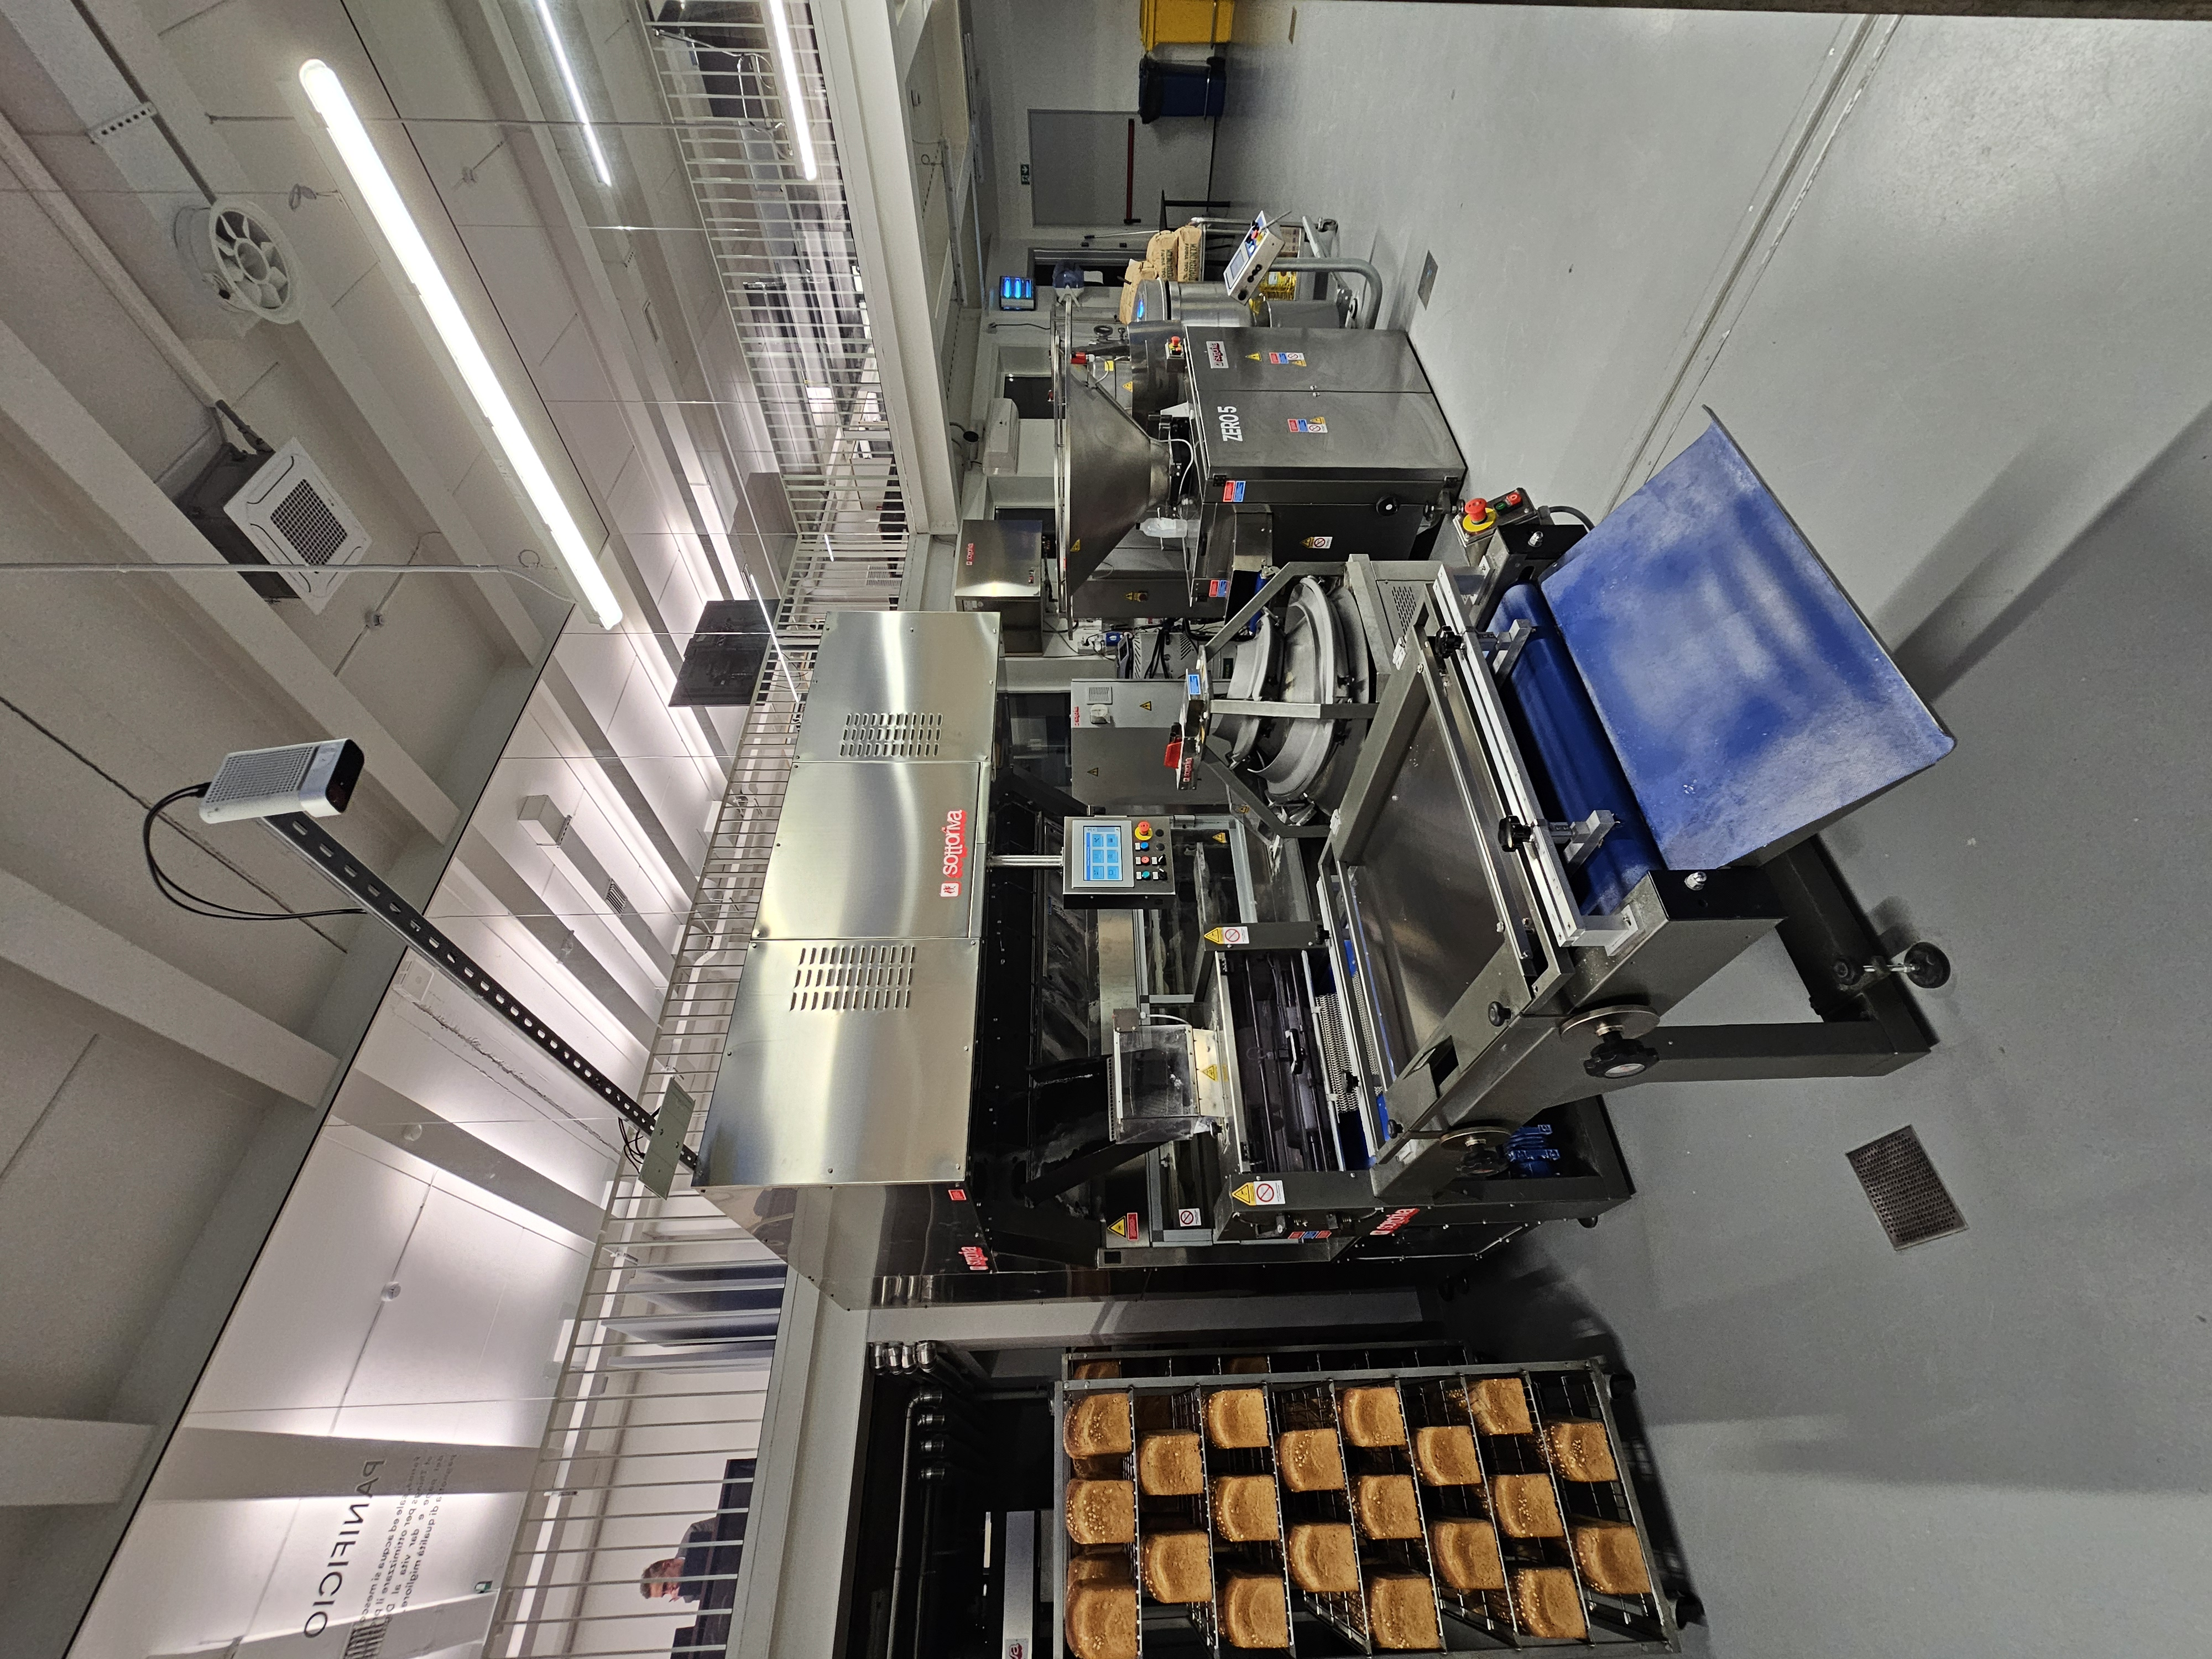
\includegraphics[scale=0.06, angle=-90, trim={0 120 120 40}, clip]{images/sito1(1).jpg}
        \caption{Automated machine pipeline at Site 1}
        \label{fig:site1_machine}
    \end{subfigure}\hfill
    \begin{subfigure}[h]{0.48\textwidth}
        \centering
        %\vspace{0pt}% allinea in alto
        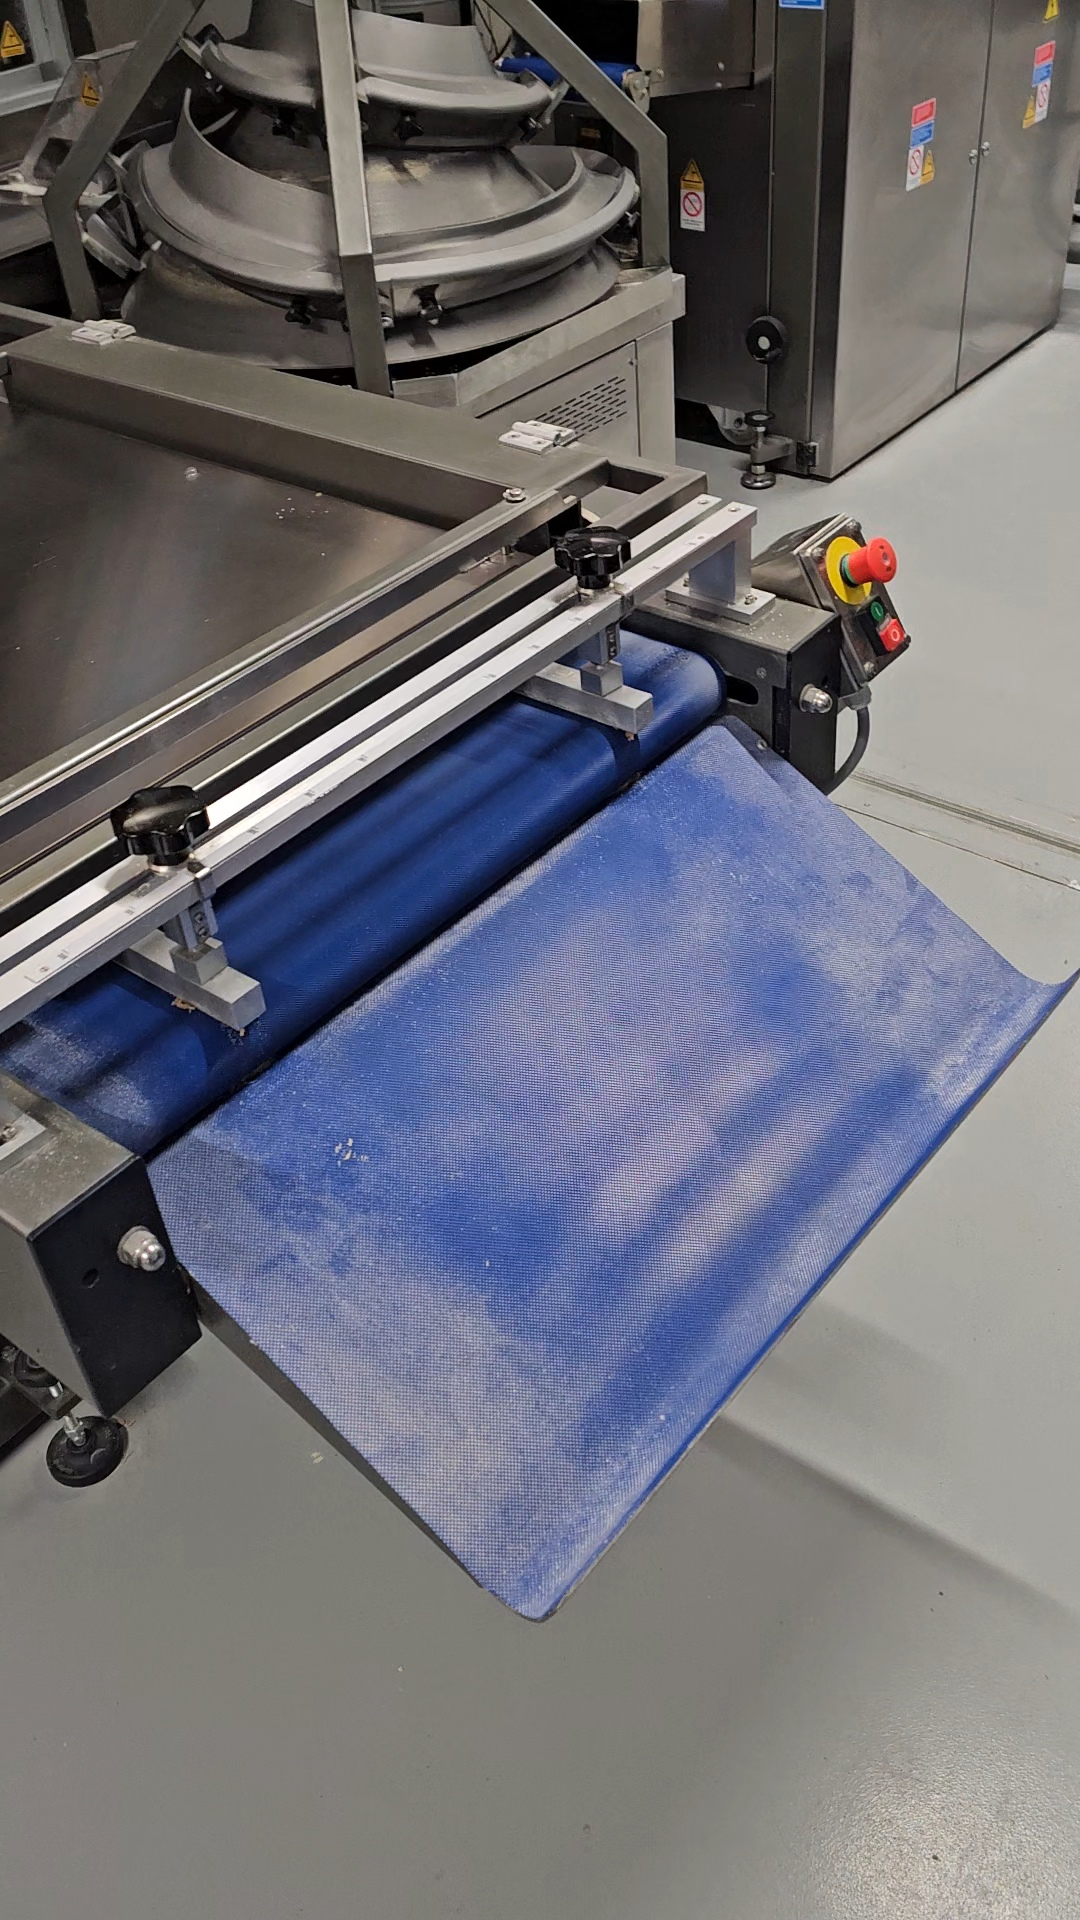
\includegraphics[scale=0.19, trim={0 280 0 400}, clip]{images/Output1-2.jpg}
        \caption{Output table where the dough balls arrive}
        \label{fig:site1_output}
    \end{subfigure}
    \caption{Overview of Site 1 and close-up of the machine output area}
    \label{fig:site1_overview}
\end{figure}
\newpage
\subsubsection{Industrial Context and Process Description}
At Site 1, the dough mixture is processed by an automated forming machine that portions and shapes the material into approximately cylindrical dough balls. These dough balls exit the machine sequentially and move along a conveyor belt until they reach the output table shown in Figure~\ref{fig:site1_output}. Variability in size and shape may occur due to fluctuations in the upstream mixing and forming processes. For quality-control purposes, it is therefore important to monitor geometric properties such as volume in a non-contact manner.

To address this requirement, a vision-based acquisition setup was installed above the machine output area, as illustrated in Figure~\ref{fig:site1_overview} and Figure~\ref{fig:hardware_site1}. The hardware configuration consists of an \emph{NVIDIA Jetson Nano 2GB Developer Kit} \cite{nvidia_corporation_jetson_nodate} for edge computation and an \emph{Azure Microsoft Kinect} RGB-D sensor \cite{microsoft_azure_nodate} for synchronized color and depth acquisition. Further details on the sensing hardware and on the Time-of-Flight principle are provided in the dedicated subsections of this chapter.

\begin{figure}[h]
    \centering
    \begin{subfigure}[h]{0.48\textwidth}
        \centering
        %\vspace{0pt}% allinea in alto
        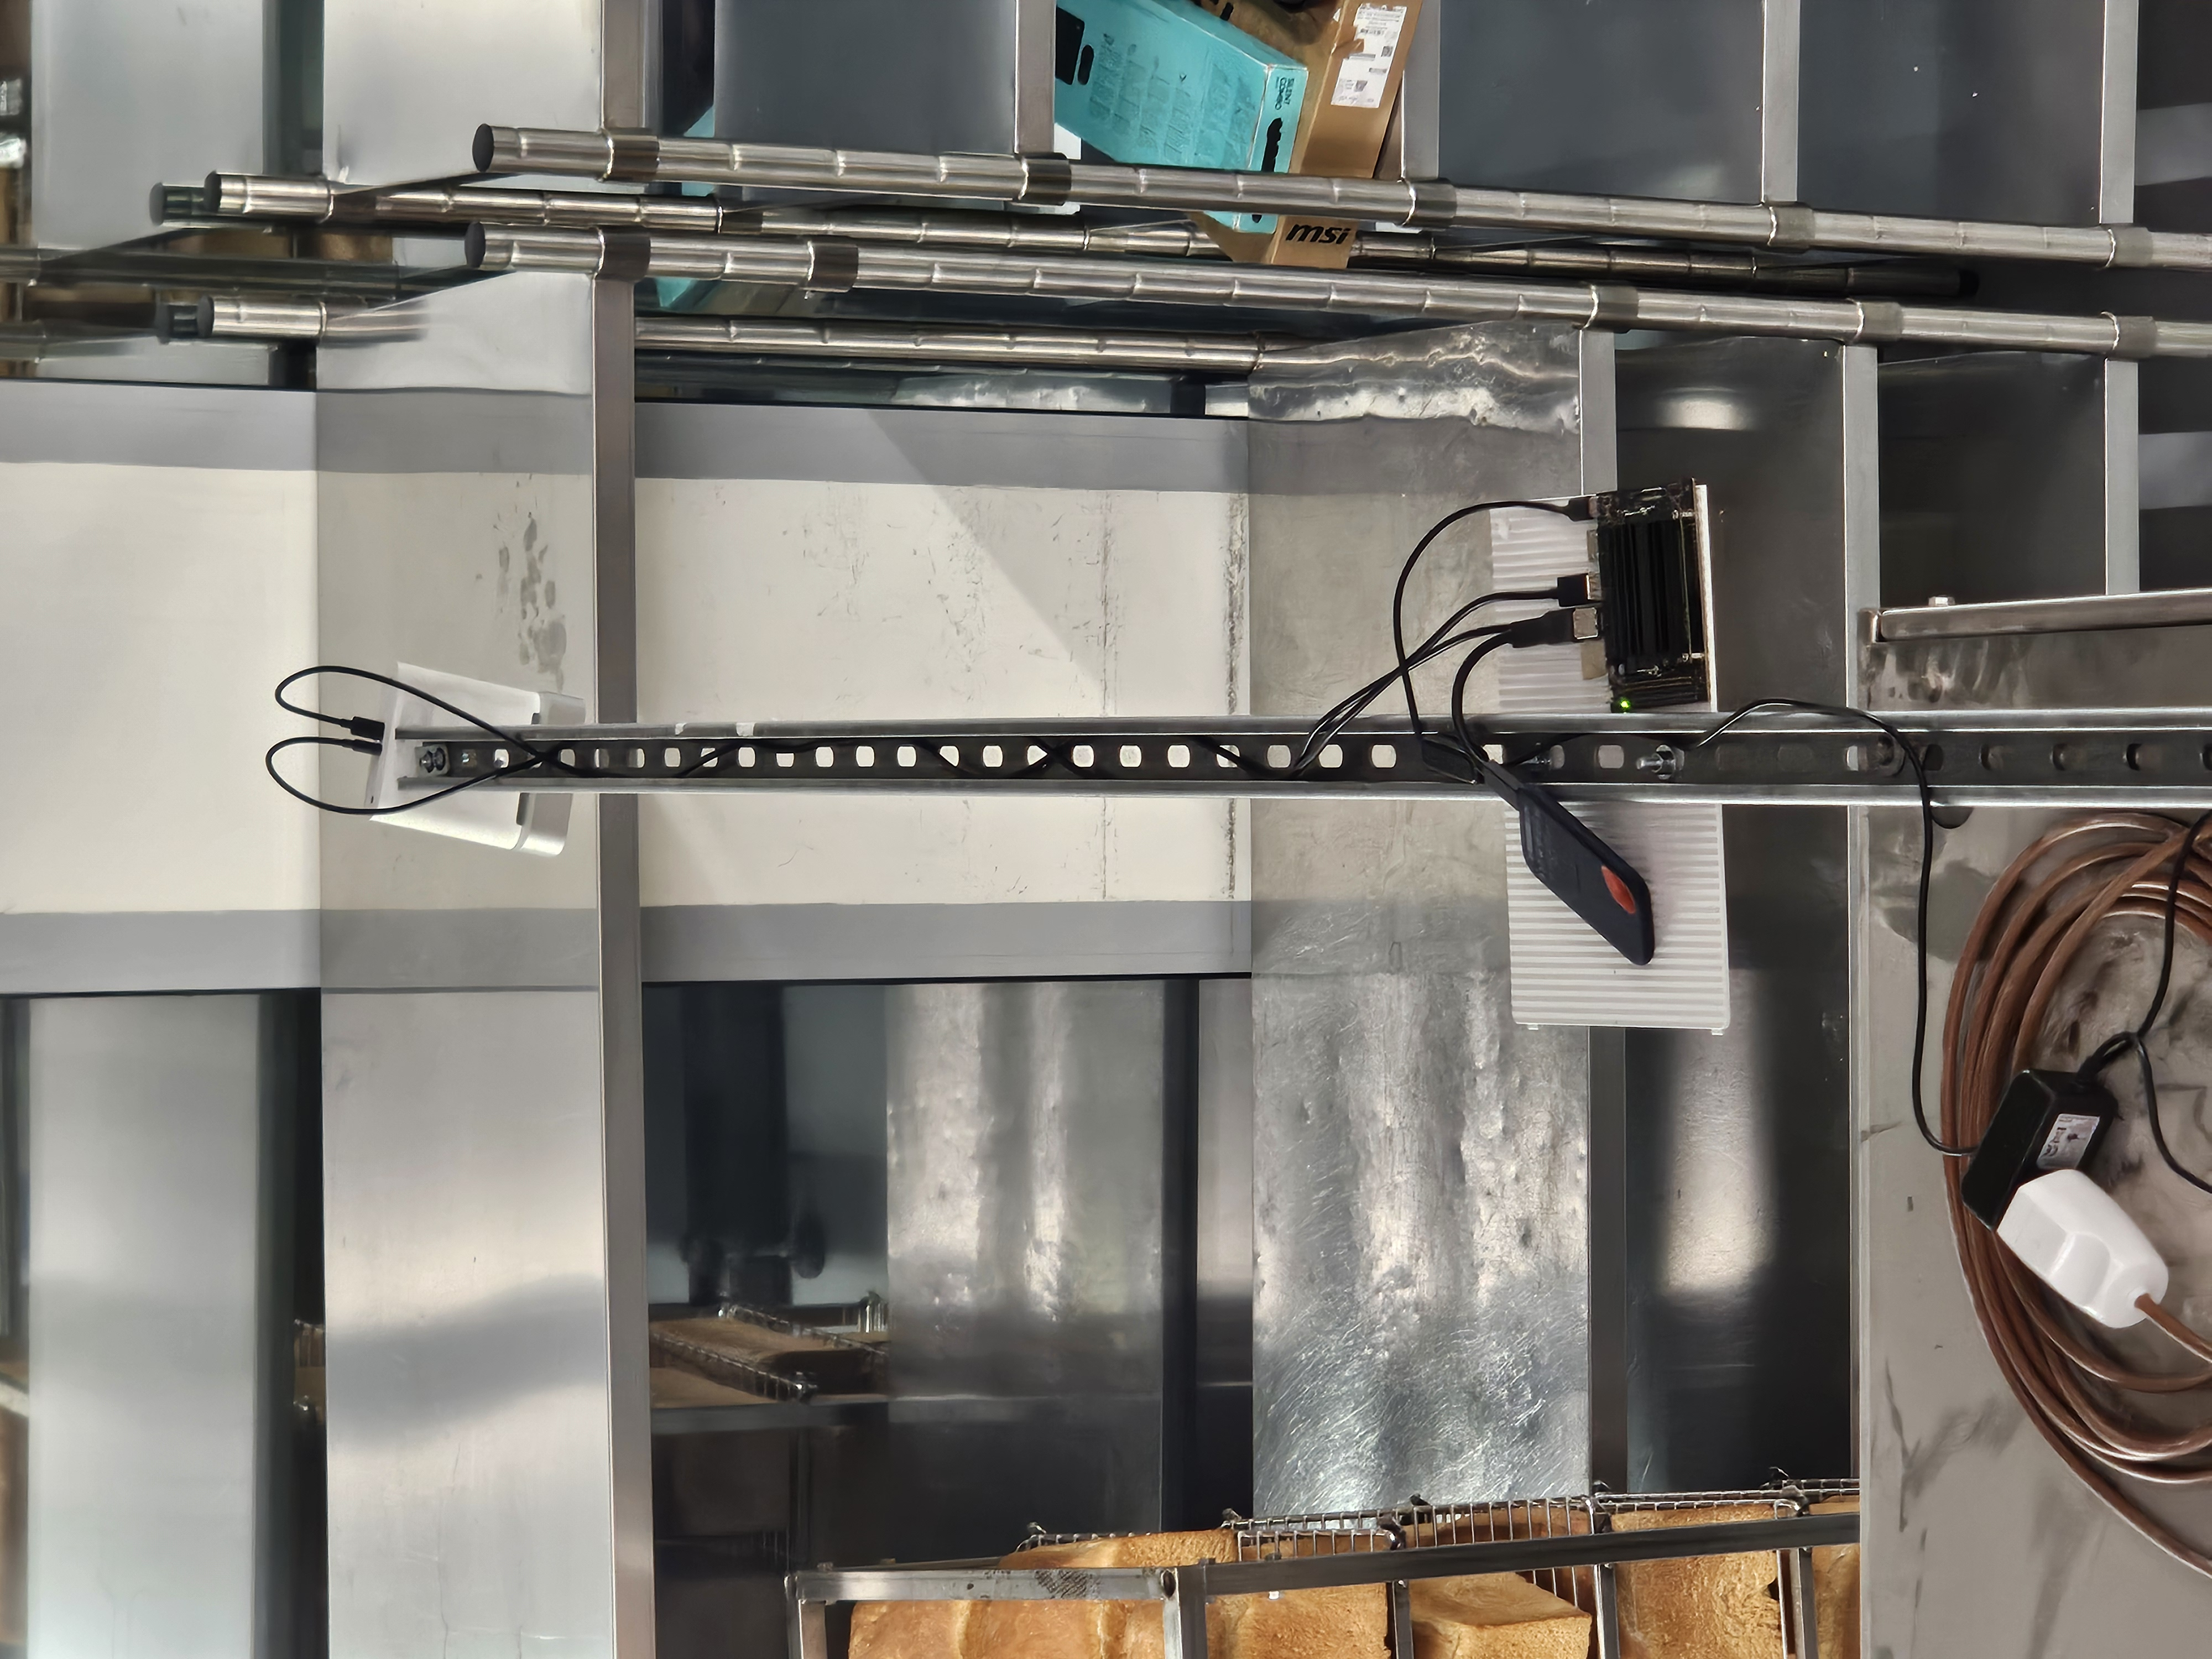
\includegraphics[width=\textwidth, angle=-90]{images/Jetson+Kinect.jpg}
        \caption{Jetson Nano and Azure Kinect used in the Site 1 setup}
    \end{subfigure}
    \begin{subfigure}[h]{0.48\textwidth}
        \centering
        %\vspace{0pt}% allinea in alto
        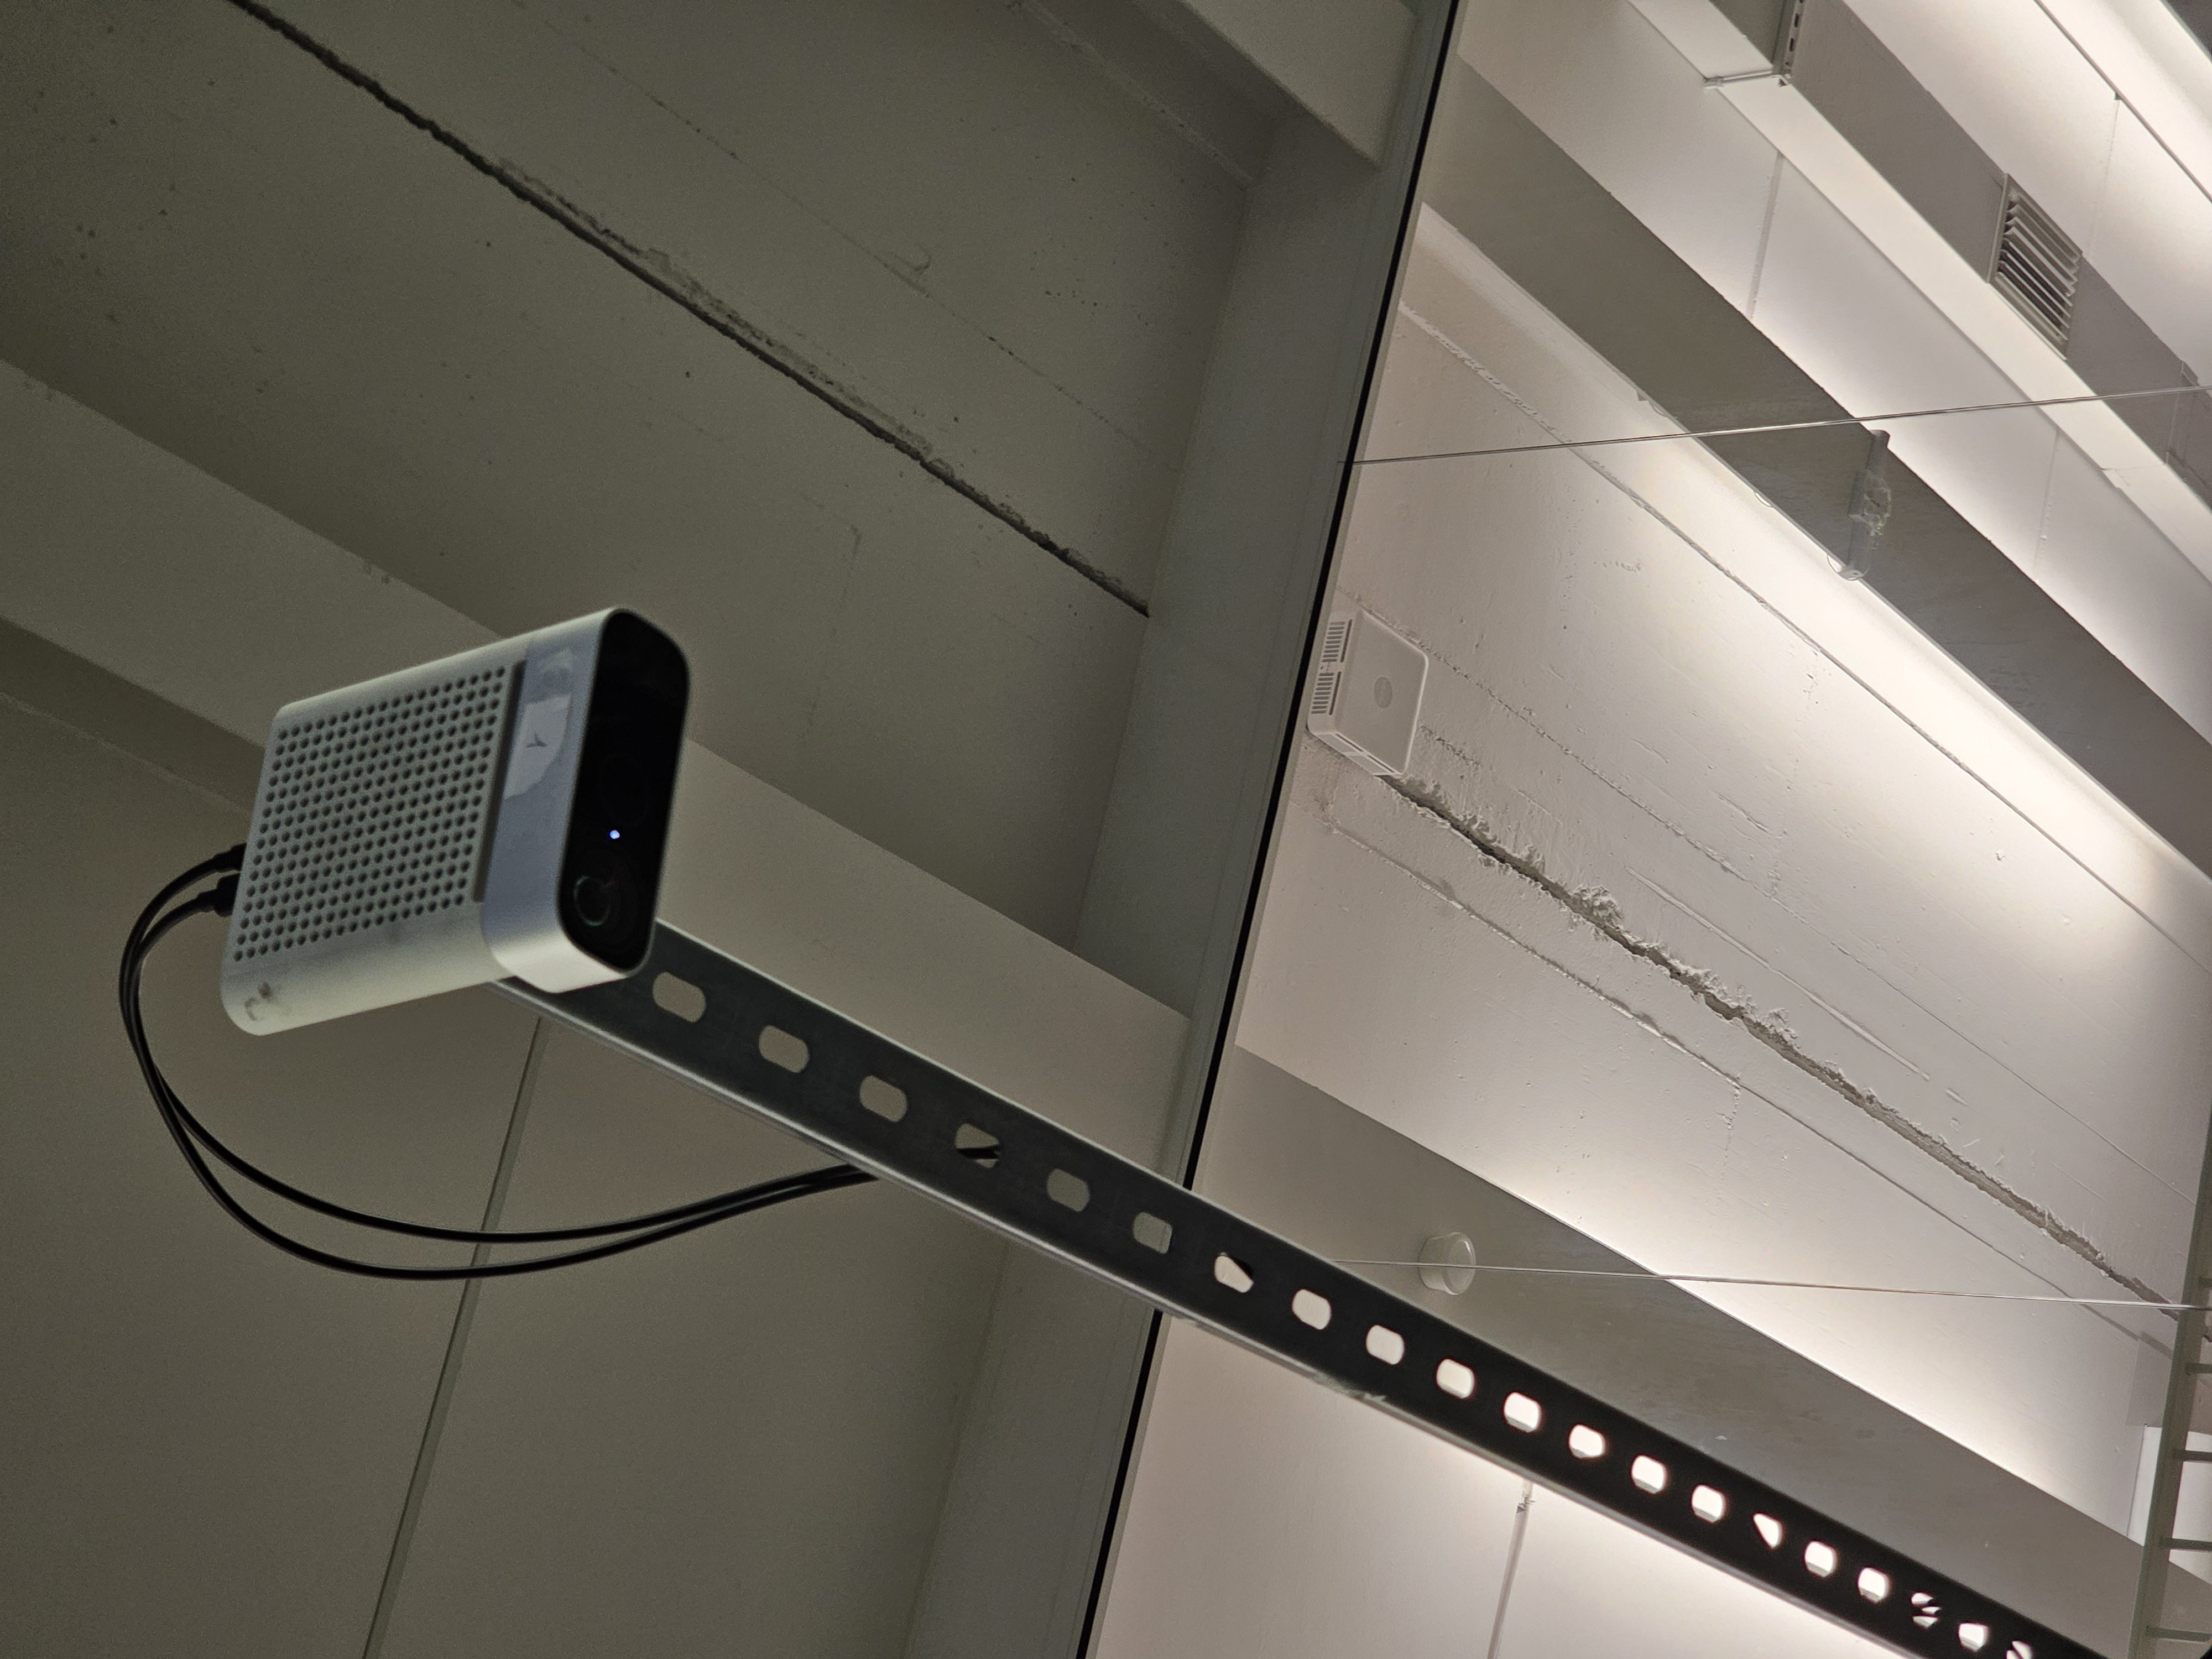
\includegraphics[width=\textwidth, angle=-90]{images/Kinect_on_site1.jpg}
        \caption{Azure Kinect mounted above the machine output area}
    \end{subfigure}
    \caption{Hardware configuration at Site 1, showing the Jetson Nano and the Azure Kinect mounted above the machine output area for RGB-D acquisition of the dough balls shown in Figure~\ref{fig:site1_output}}
    \label{fig:hardware_site1}
\end{figure}

\subsubsection{Offline Data Acquisition}
During the offline phase, the system operates in data acquisition mode. In this configuration, the Azure Kinect continuously captures synchronized RGB and depth frames. A motion detection algorithm is executed on the Jetson Nano to identify pixel variations in the scene corresponding to the passage of dough balls under the camera.

The motion detection module serves exclusively as a trigger mechanism for dataset collection. When motion is detected within a predefined and configurable region of interest (ROI), the corresponding RGB-D frame is stored. In this setup, the ROI was defined so as to cover the entire machine output area (shown in Figure~\ref{fig:site1_output}).
\newpage
This approach ensures that:
\begin{itemize}
    \item only relevant frames containing dough balls are acquired;
    \item redundant background movement is discarded;
    \item the dataset remains balanced and computationally manageable.
\end{itemize}
\begin{figure}[h]
    \centering
    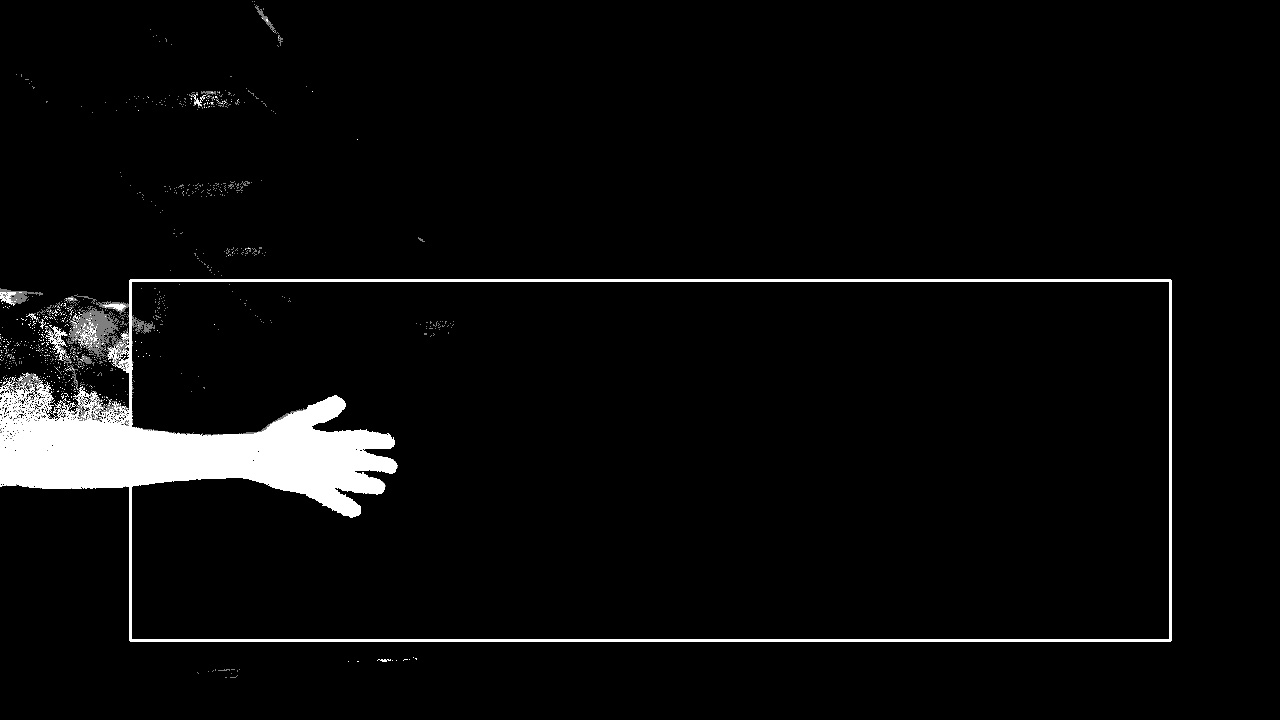
\includegraphics[width=0.65\linewidth]{images/ROI_example.jpg}
    \caption{Example of a configurable region of interest (ROI) superimposed on a background-subtraction mask. Although this example refers to the Site~2 workstation shown in Figure~\ref{fig:breadloaf}, it illustrates the same motion-triggering principle adopted for data acquisition at both sites. The white region corresponds to the detected foreground, while the black region represents the background.}
    \label{fig:acquisition_site1}
\end{figure}
The collected dataset is subsequently annotated through an automatic labelling strategy based on Language Segment-Anything \cite{medeiros_luca-medeiroslang-segment-anything_2026}, and the resulting annotations are then used to train the DEIMv2 object detection network in an offline environment. The details of the labelling procedure and training setup are presented in Chapter~4.

\begin{figure}[h]
    \centering
    
\includegraphics[width=0.55\linewidth]{images/motion_detection.jpg}
    \caption{Example of the motion detection module at Site~1, showing a dough ball passing through the monitored area and activating the trigger used to store the corresponding RGB-D frame for dataset creation.}
    \label{fig:motion_detection}
\end{figure}

\subsubsection{Online Inference and Volume-Oriented Processing}

After training, the system is deployed online at Site 1 using the same hardware configuration, namely the Jetson Nano and the Azure Kinect. In the online phase, the trained DEIMv2 network detects the dough balls directly in the RGB stream, while the aligned depth data provide the spatial information required for volumetric analysis.

The detected regions are therefore converted into local 3D representations and further processed to estimate dough volume. The detailed processing pipeline, including point-cloud generation, background removal, 3D completion, and final volume estimation, is described in Chapter~4.

\subsubsection{System Objectives at Site 1}

The implementation at Site 1 serves as a proof-of-concept for an edge-based RGB-D inspection system capable of:

\begin{itemize}
    \item automated dataset acquisition in industrial conditions;
    \item real-time object detection on embedded hardware;
    \item 3D reconstruction from RGB-D data;
    \item Non-contact volumetric estimation of deformable food products.
\end{itemize}

The modular design adopted at Site~1 ensures that the same sensing and computational infrastructure can be reused across both offline training and online inference phases. More generally, the same acquisition philosophy based on edge computing, motion-triggered capture, and downstream visual analysis is also maintained at Site~2, thereby minimizing hardware complexity and deployment costs across the overall framework.
